\documentclass[12pt,fleqn]{article}\usepackage{../../common}
\begin{document}
Ders 31

Önceki derste dolam (curl) kavramını işledik, bir vektör alanının dönüşünü
hesaplıyordu, elde edilen vektörün yönü dönüş yönü, vektörün büyüklüğü ise
açısal hızın iki katı idi.

Örnek olarak alttaki alanlara bakalım,

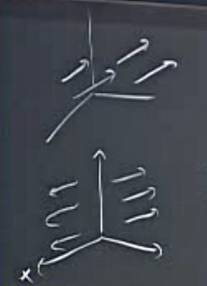
\includegraphics[width=10em]{calc_multi_31_01.jpg}

Figürlerden birincisi $\vec{F} = < a,b,c > $ diyelim, sabit bir vektör
alanı, her noktada aynı hızda yer değişim var, burada dönüş göremiyoruz.
Bu alan üzerinde dolam hesabı yaparken bir sürü kısmı türev alınacak tabii,
ve sabit değerlerin türevleri sıfır olacağı için $\curl \vec{F} = 0$ olur.

İkinci figürde $x$ ekseni boyunca esnetme yapan bir görülüyor, tüm gidişat
$x$'e paralel, diyelim $\vec{F} = < x, 0, 0 >$. Bu alanın dolamı yine sıfır.
Dolam esneme gibi kavramları ölçemez, uzaklaşım (divergence) bunu yapabilirdi,
ama elde hala dönüş yok, demek ki dolam da yok.





[devam edecek]

Kaynaklar

\end{document}
